\documentclass[12pt,a4paper]{article}
\usepackage{amsmath,amsfonts,amssymb}
\usepackage{graphicx}
\usepackage{enumitem}
\usepackage[dvipsnames]{xcolor}
\usepackage{pgfplots}
\usepackage{hyperref}
\usepackage{soul}
\usepackage{framed}
\usepackage{booktabs} 
\usepackage{tabularx}
\usepackage{array}


\definecolor{lessonbgcolor}{rgb}{0.9,0.9,1}
\definecolor{examplecolor}{rgb}{0.8,1,0.8}
\definecolor{noteboxcolor}{rgb}{1,0.8,0.8}
\newenvironment{lesson}[1]
  {\begin{framed}\colorbox{lessonbgcolor}{
  \parbox{\dimexpr\linewidth-2\fboxsep}{
  \textbf{#1}}}\end{framed}}
  
\newenvironment{example}
  {\begin{framed}\colorbox{examplecolor}{
  \parbox{\dimexpr\linewidth-2\fboxsep}{
  \textbf{Example:}}}}
  {\end{framed}}
\newenvironment{note}
  {\begin{framed}\colorbox{noteboxcolor}{
  \parbox{\dimexpr\linewidth-2\fboxsep}{
  \textbf{Note:}}}}
  {\end{framed}}

\pgfplotsset{width=7cm,compat=1.17}
\begin{document}
\section*{Unit 4: Exponential Functions}
\begin{lesson}{1 - Exponential Growth}
\textcolor{blue}{Exponential growth} is a captivating concept where a quantity increases at a fixed percentage rate over time. This growth is modeled by the formula $y = ab^x$, where $a$ is the initial amount, $b$ is the growth factor, and $x$ is the time variable.

\begin{example}
Suppose you invest $1000$ at an annual interest rate of $5\%$, compounded annually. The growth formula is $A = 1000 \times (1 + 0.05)^x$. After 3 years, the amount would be approximately $A = 1000 \times (1 + 0.05)^3 \approx 1157.63$.
\end{example}

\begin{note}
The graph of an exponential growth function is characterized by a distinct upward curve that becomes steeper as $b$ increases.

\begin{center}
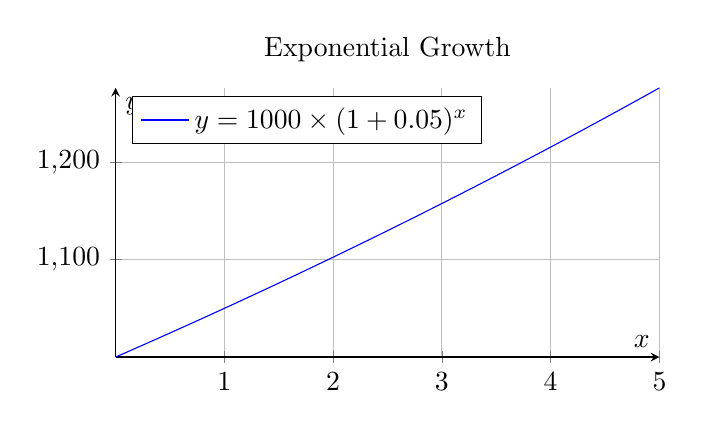
\begin{tikzpicture}
\begin{axis}[
  xlabel=$x$,
  ylabel=$y$,
  grid=major,
  axis lines=middle,
  width=0.7\linewidth,
  height=5cm,
  title={Exponential Growth},
  legend pos=north west,
]
\addplot[blue, domain=0:5, samples=100, smooth] {1000 * (1 + 0.05)^x};
\addlegendentry{$y = 1000 \times (1 + 0.05)^x$}
\end{axis}
\end{tikzpicture}
\end{center}
\end{note}
\end{lesson}
\newpage
\begin{lesson}{2 - Exponential Decay}
\textcolor{blue}{Exponential decay} is the counterpart to exponential growth. It occurs when a quantity decreases at a fixed percentage rate over time. The decay is modeled by the formula $y = ab^x$, where $b$ is between 0 and 1.

\begin{example}
Consider a radioactive substance that decays at a rate of 10\% per year. Its decay formula is $N = N_0 \times 0.9^t$. After 5 years, the remaining quantity is $N = N_0 \times 0.9^5$.
\end{example}

\begin{note}
The graph of an exponential decay function exhibits a decreasing curve that approaches but never reaches zero.

\begin{center}
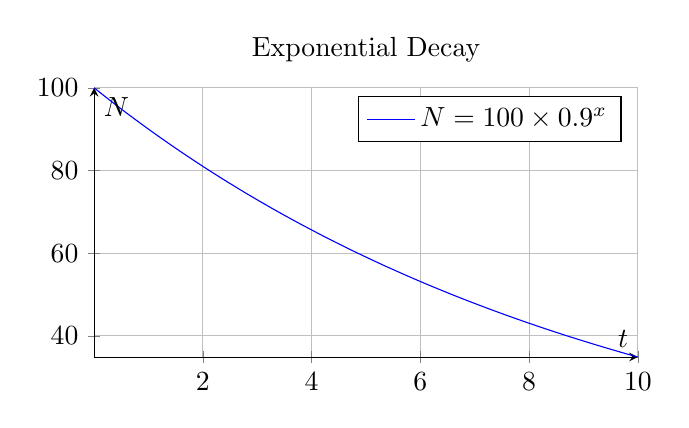
\begin{tikzpicture}
\begin{axis}[
  xlabel=$t$,
  ylabel=$N$,
  grid=major,
  axis lines=middle,
  width=0.7\linewidth,
  height=5cm,
  title={Exponential Decay},
  legend pos=north east,
]
\addplot[blue, domain=0:10, samples=100, smooth] {100 * 0.9^x};
\addlegendentry{$N = 100 \times 0.9^x$}
\end{axis}
\end{tikzpicture}
\end{center}
\end{note}
\end{lesson}
\newpage
\begin{lesson}{3 - Compound Interest}
\textcolor{blue}{Compound interest} is a powerful concept where interest is added to the initial principal, which then earns interest over time. The compound interest formula is given by $A = P(1 + r/n)^{nt}$, where $A$ is the final amount, $P$ is the principal, $r$ is the annual interest rate, $n$ is the number of times interest is compounded per year, and $t$ is the time in years.

\begin{example}
Imagine investing $5000$ at an annual interest rate of $6\%$, compounded quarterly. The formula is $A = 5000 \times (1 + 0.06/4)^{4t}$. After 2 years, the amount is $A = 5000 \times (1 + 0.06/4)^{4 \times 2}$.
\end{example}

\begin{note}
Compound interest enables your investment to grow faster compared to simple interest, especially with more frequent compounding.
\end{note}
\end{lesson}
\newpage 
\begin{lesson}{4 - Properties of Exponential Functions}
\textcolor{blue}{Exponential functions} possess several key properties:

\begin{itemize}
    \item They have a constant base.
    \item They can model growth or decay.
    \item They have an asymptote, which they approach but never reach.
    \item They are always positive if the base is greater than 1.
    \item They are always decreasing if the base is between 0 and 1.
\end{itemize}

\begin{example}
Consider the function $f(x) = 2^x$. It has a constant base of 2 and models exponential growth.
\end{example}

\begin{note}
The graph of an exponential function approaches but never crosses the horizontal axis (asymptote).

\begin{center}
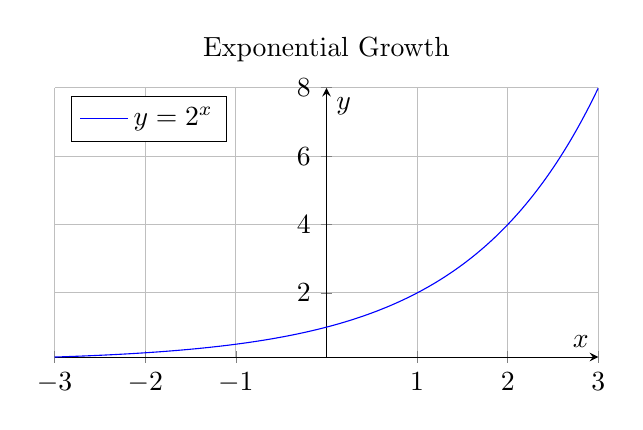
\begin{tikzpicture}
\begin{axis}[
  xlabel=$x$,
  ylabel=$y$,
  grid=major,
  axis lines=middle,
  width=0.7\linewidth,
  height=5cm,
  title={Exponential Growth},
  legend pos=north west,
]
\addplot[blue, domain=-3:3, samples=100, smooth] {2^x};
\addlegendentry{$y = 2^x$}
\end{axis}
\end{tikzpicture}
\end{center}
\end{note}
\end{lesson}
\newpage 
\begin{lesson}{5 - Transformations}
\textcolor{blue}{Transformations} offer a way to modify the graph of an exponential function. Common transformations include vertical shifts, horizontal shifts, reflections, and stretches or compressions. These transformations are applied to the base function $y = b^x$.

\begin{example}
If $g(x) = 3 \times 2^x$, the function $g$ is a vertical stretch of $f(x) = 2^x$ by a factor of 3.
\end{example}

\begin{note}
Transformations alter the appearance and behavior of the exponential function graph.

\begin{center}
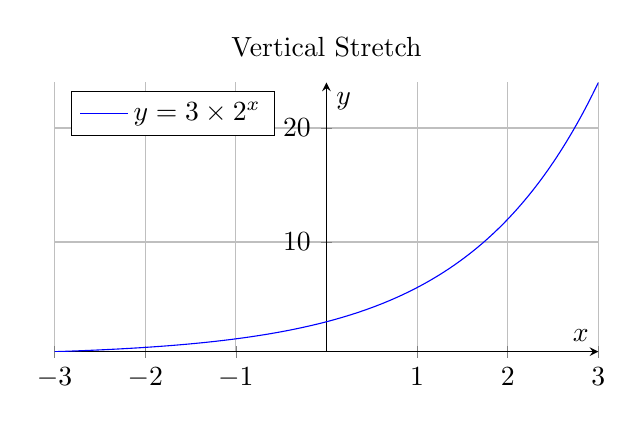
\begin{tikzpicture}
\begin{axis}[
  xlabel=$x$,
  ylabel=$y$,
  grid=major,
  axis lines=middle,
  width=0.7\linewidth,
  height=5cm,
  title={Vertical Stretch},
  legend pos=north west,
]
\addplot[blue, domain=-3:3, samples=100, smooth] {3 * 2^x};
\addlegendentry{$y = 3 \times 2^x$}
\end{axis}
\end{tikzpicture}
\end{center}
Transformations can also involve horizontal shifts, reflections, and other modifications to customize the behavior of the exponential function graph.
\end{note}
\end{lesson}



\newpage
\begin{lesson}{6 - Applications of Exponential Functions}
\textcolor{blue}{Exponential functions} find applications in various real-world scenarios, such as population growth, radioactive decay, and financial investments. Understanding these applications is crucial for solving problems in science, economics, and other fields.

\begin{example}
Population growth can be modeled using the exponential function $P(t) = P_0 \times (1 + r)^t$, where $P(t)$ is the population at time $t$, $P_0$ is the initial population, $r$ is the growth rate, and $t$ is time.
\end{example}

\begin{example}
Radioactive decay is a common application where the decay of a substance is modeled by the function $N(t) = N_0 \times e^{-kt}$, where $N(t)$ is the remaining quantity at time $t$, $N_0$ is the initial quantity, $k$ is the decay constant, and $t$ is time.
\end{example}

\begin{example}
Financial investments often involve compound interest, and the amount of money accumulated over time is given by the formula $A = P(1 + r/n)^{nt}$, where $A$ is the final amount, $P$ is the principal, $r$ is the annual interest rate, $n$ is the number of times interest is compounded per year, and $t$ is time in years.
\end{example}
\end{lesson}
\newpage
\begin{lesson}{7 - Summative Assessment }
\begin{enumerate}
    \item \textbf{Evaluate the following:}
    \begin{enumerate}[label=\alph*)]
        \item $2^3$:
        \begin{align*}
            2^3 &= 2 \times 2 \times 2 \\
            &= 8
        \end{align*}
        
        \item $10^{-2}$:
        \begin{align*}
            10^{-2} &= \frac{1}{10^2} \\
            &= \frac{1}{100} \\
            &= 0.01
        \end{align*}
        
        \item $e^0$:
        \begin{align*}
            e^0 &= 1
        \end{align*}
    \end{enumerate}
    
    \item \textbf{Solve for $x$:}
    \begin{enumerate}[label=\alph*)]
        \item $5^x = 125$:
        \begin{align*}
            5^x &= 125 \\
            x &= 3
        \end{align*}
        
        \item $2e^{2x} = 16$:
        \begin{align*}
            e^{2x} &= 8 \\
            2x &= \ln(8) \\
            x &= \frac{\ln(8)}{2}
        \end{align*}
    \end{enumerate}
\newpage
    \item \textbf{Consider the function $f(x) = 3 \times 2^x$. Perform the following transformations and sketch the resulting graph:}
    \begin{enumerate}[label=\alph*)]
        \item \textbf{Vertical stretch by a factor of 2:}
        The function becomes $g(x) = 6 \times 2^x$.
        
        \item \textbf{Horizontal shift right by 1 unit:}
        The function becomes $h(x) = 3 \times 2^{(x - 1)}$.
        
        \item \textbf{Reflection across the $x$-axis:}
        The function becomes $k(x) = -3 \times 2^x$.
        
        \textbf{Graph:} (Note: This is a conceptual sketch; precise plotting requires numerical values.)

\definecolor{lessonbgcolor}{rgb}{0.9,0.9,1}
\definecolor{examplecolor}{rgb}{0.8,1,0.8}
\definecolor{blue}{RGB}{0,70,170}

\pgfplotsset{
    compat=1.17,
    every axis/.append style={
        axis line style={->},
        xlabel style={anchor=west},
        ylabel style={anchor=south},
        legend style={at={(0.03,0.97)}, anchor=north west, draw=none, fill=none, font=\scriptsize},
    },
}


\begin{figure}[h]
    \centering
    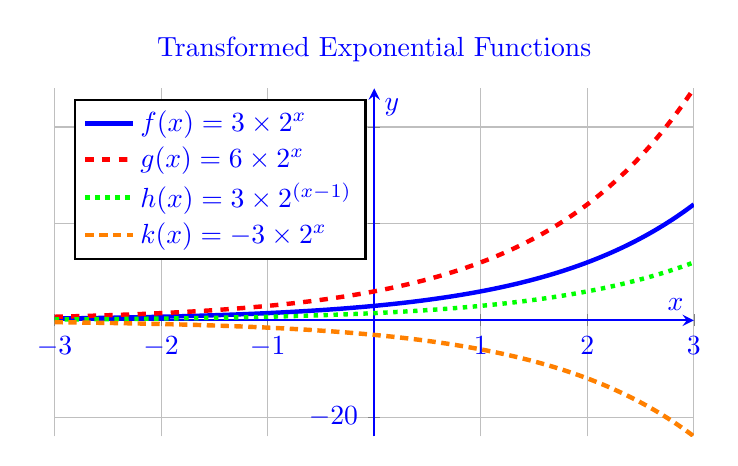
\begin{tikzpicture}
        \begin{axis}[
            xlabel={$x$},
            ylabel={$y$},
            grid=major,
            axis lines=middle,
            width=0.8\linewidth,
            height=6cm,
            title={Transformed Exponential Functions},
            legend pos=north west,
            domain=-3:3,
            samples=100,
            smooth,
            % Adjust the style of each plot
            blue,
            thick,
            every axis plot/.append style={ultra thick},
            legend cell align=left,
        ]
            \addplot [blue] {3 * 2^x};
            \addlegendentry{$f(x) = 3 \times 2^x$}
            
            \addplot [red, dashed] {6 * 2^x};
            \addlegendentry{$g(x) = 6 \times 2^x$}
            
            \addplot [green, dotted] {3 * 2^(x - 1)};
            \addlegendentry{$h(x) = 3 \times 2^{(x - 1)}$}
            
            \addplot [orange, densely dashed] {-3 * 2^x};
            \addlegendentry{$k(x) = -3 \times 2^x$}
        \end{axis}
    \end{tikzpicture}
    \caption{Transformed Exponential Functions}
    \label{fig:transformed-exponential}
\end{figure}
    \end{enumerate}
\end{enumerate}
\end{lesson}
\end{document}
